\section{Datentransformation}
\label{dt}
Die Daten -- in Form von Schüssen -- wurden selektiert, bereinigt und anschließend auf eine relevante Zielmenge reduziert. In dieser Phase müssen diese Daten nur noch in eine adaptierte Form für die anschließende Regressionsanalyse transformiert werden, wozu einige der in \vref{dt} vorgestellten Methoden ihre Verwendung finden. Nachfolgend werden allgemeine Transformationen (vgl. \vref{at}), wie die des Koordinatensystems, sowie speziell für die Betrachtungswinkel (vgl. \vref{wdt} und \vref{kt}) ausgerichtete Transformationen durchgeführt, um ein passendes Format für die Verarbeitung in \gls{matlab} bereitstellen zu können.


\subsection{Allgemeine Transformationen}
\label{at}
Im Folgenden werden die allgemeinen Transformationen betrachtet, welche sowohl für die Betrachtung des Winkels- und der Distanz als auch in Bezug auf die Koordinaten notwendig sind.

\paragraph{Unterscheidung zwischen Tor und Nicht-Tor} Nach der Datenreduzierung liegen die Datensätze wie in \vref{redData} abgebildeten Format vor, wobei die \textsf{type\_id} Aufschluss über das Resultat des Schusses gibt. Aus der \Vref{tab:events} lässt sich entnehmen, dass die Type-IDs \textsf{13, 14} und \textsf{15} einen Schuss ohne Torerfolg widerspiegeln, sowie die Type-ID \textsf{16} einen Torerfolg. Demzufolge wird das Attribut \textsf{type\_id} durch eine \textit{Codierung} in das Attribut \textsf{goal} transformiert, welches die Werte \textsf{0} für \textbf{Nicht-Tor} und \textsf{1} für \textbf{Tor}, in Form eines numerischen Wertes, übernimmt. \vref{atData} zeigt dazu exemplarisch das adaptierte Format der Schüsse aus \vref{redData}.

\paragraph{Transformation des Koordinatensystems}
Aus Anforderung 6 (vgl. \vref{tab:anf}) geht hervor, dass der Ursprungspunkt $P(0|0)$ der Funktion in der Mitte der gegnerischen Torauslinie liegen muss, sodass eine Transformation des Koordinatensystems nötig ist. Der Ursprungspunkt $P(0|0)$ liegt im  vorgegebenen Koordinatensystem von Opta (siehe \vref{opta_pitch}) in der eigenen Spielhälfte (links) auf dem unteren Eckstoßpunkt und muss, wie in \vref{transf_pitch} dargestellt, verschoben werden. Zusätzlich werden die Achsen umgekehrt, wodurch sich folgende Transformation der x- und y-Koordinate ergibt:\enlargethispage{\baselineskip}\newline

\centerline{$\boldsymbol{x_{neu}} \Rightarrow$ y - 50 }
\centerline{$\boldsymbol{y_{neu}} \Rightarrow$ |x - 100|}

Dafür wird ebenfalls die Codierung angewendet, um der x-Koordinate in Abhängigkeit der y-Koordinate (und umgedreht) mit zusätzlicher Verschiebung einen neuen Wert, nun numerisch, zuzuweisen. Da beide Koordinatenwerte gleich skaliert sind, ist in diesem Fall keine \textit{Normalisierung} der Attribute notwendig.

\begin{figure}[H]
\centering
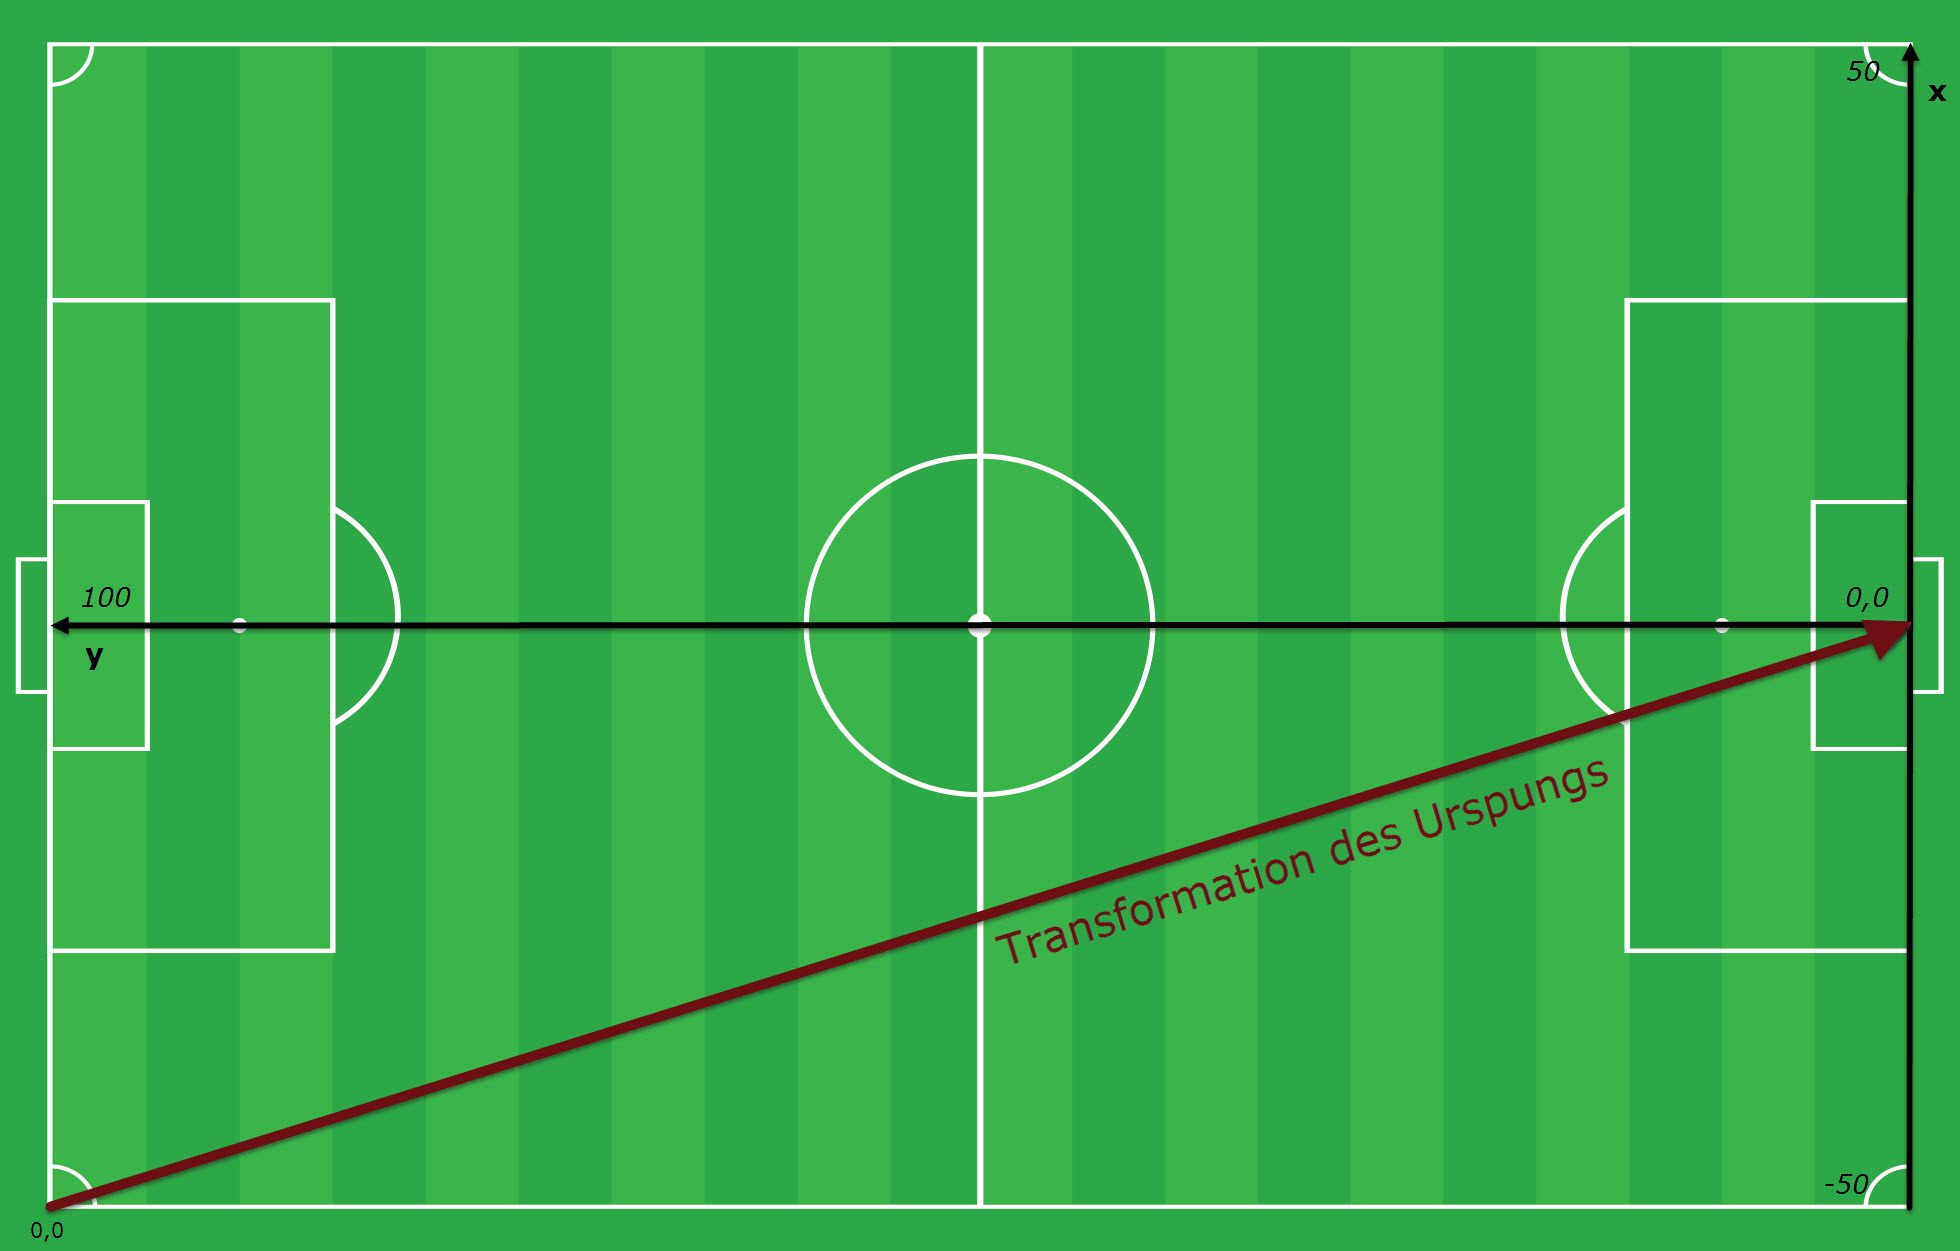
\includegraphics[scale=0.27]{se-wa-jpg/transf_pitch}
\caption[Transformation des Koordinatensystems]{Transformation des Koordinatensystems}
\label{transf_pitch}
\end{figure}

\enlargethispage{2\baselineskip} Folglich ergibt sich nach diesen Transformationen eine neue Struktur der Datensätze, die in Bezug auf die Daten aus \vref{redData} in \vref{atData} dargestellt sind.\newline

\captionListing{Struktur der Daten nach der allgemeinen Transformation}
\begin{lstlisting}[caption=\captionListingText,language=json,xleftmargin=5mm,label=atData] 
[
	{
		"goal": 1,
		"x": -6.5,
		"y": 5
	},
	{
		"goal": 0,
		"x": 25.9,
		"y": 10.8,
	},
	...
]
\end{lstlisting}



\subsection{Transformation für Winkel- und Distanzbetrachtung}
\label{wdt}
Für eine Betrachtung der Wahrscheinlichkeit für einen Torerfolg in Bezug auf die

\begin{equation}
Distanz= \sqrt{x^2 + y^2}
\end{equation}

\begin{equation}
Winkel= \arctan(\frac{|x|}{y})
\end{equation}


\begin{figure}[H]
\centering
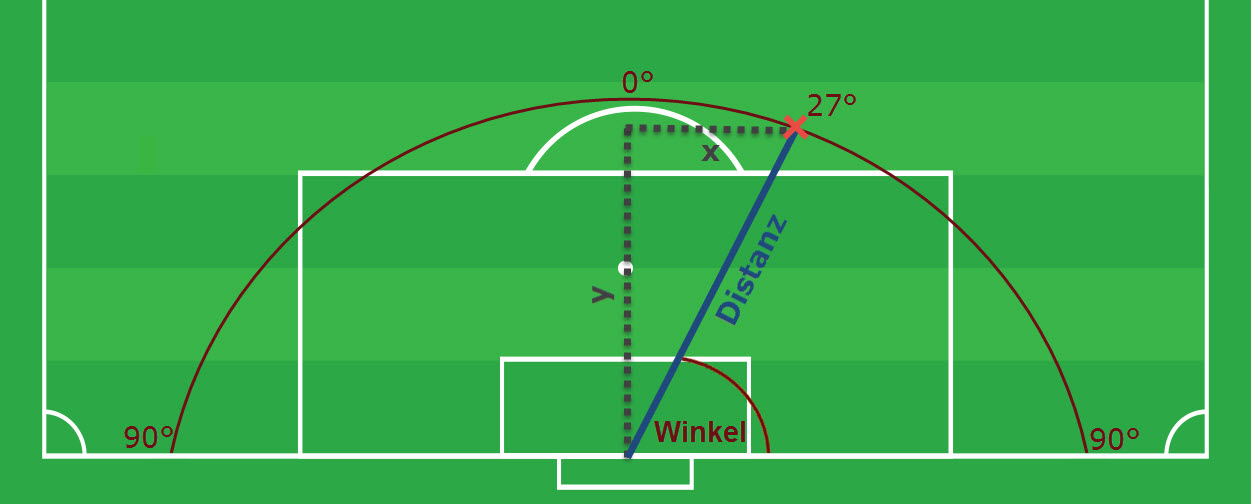
\includegraphics[scale=0.425]{se-wa-jpg/winkel_distanz}
\caption[Berechnung der Distanz und des Winkels]{Berechnung der Distanz und des Winkels}
\label{transf_pitch}
\end{figure}

\captionListing{Struktur der Daten für die Winkel- und Distanzbetrachtung}
\begin{lstlisting}[caption=\captionListingText,language=json,xleftmargin=5mm,label=wdData] 
[
	{
		"goal": 1,
		"angle": 52.4,
		"distance": 8.2
	},
	{
		"goal": 0,
		"angle": 67.4,
		"distance": 28.1,
	},
	...
]
\end{lstlisting}

\begin{itemize}
\item Winkel berechnen
\item Distanz berechnen
\item Einteilung in Intervalle
\item Abbildung der Berechnung
\end{itemize}


\subsection{Transformation für Koordinatenbetrachtung}
\label{kt}
\begin{itemize}
\item Spielfeld in Quadrate einteilen $\rightarrow$ Abbildung
\item Wahrscheinlichkeit (p) für jedes Quadrat berechnen $\rightarrow \frac{Anzahl~der~Tore~im~Quadrat}{Gesamtzahl~der~Schüsse~im~Quadrat}$ 
\item Seiten des Spielfeldes an $y$-Achse ($x=0$) spiegeln $\rightarrow$ Durchschnitt der Wahrscheinlichkeiten
\item Zielformat für MATLAB vorbereiten ($x|y|p$)
\end{itemize}

\begin{equation}
p = \frac{Anzahl~der~Tore~im~Quadrat}{Gesamtzahl~der~Schüsse~im~Quadrat}
\end{equation}

\begin{figure}[H]
\centering
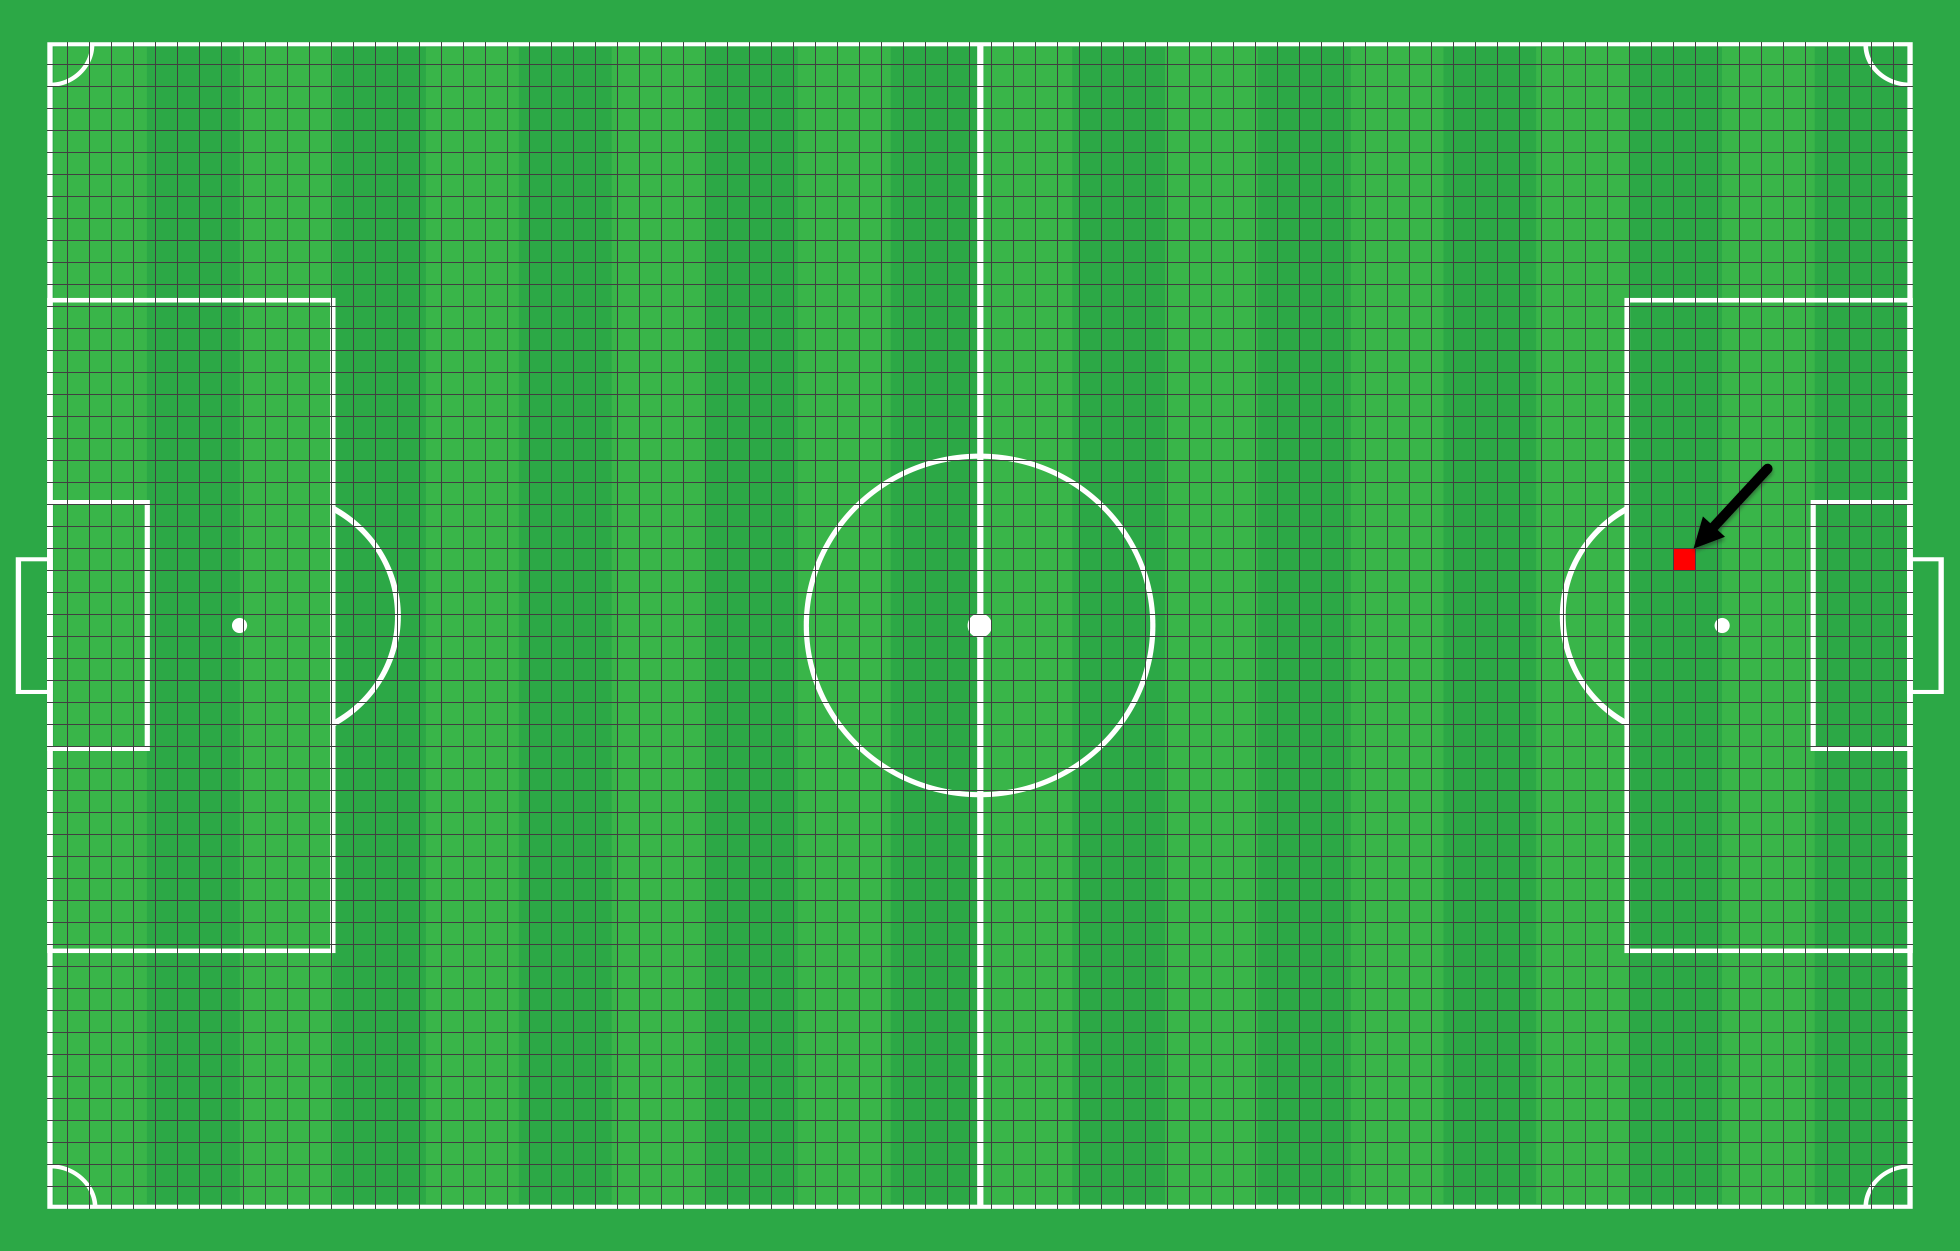
\includegraphics[scale=0.28]{se-wa-jpg/raster}
\caption[Einteilung des Spielfeldes in Raster]{Einteilung des Spielfeldes in Raster}
\label{transf_pitch}
\end{figure}

